\documentclass{article}
\usepackage{graphicx}
\usepackage{sidecap}
\title{Cpppc Project: Microfluidic-Large-Scale-Integration (mLSI) Simulator}
\author{Mengchu Li}
\begin{document}
\maketitle
\section{Introduction}

Microfluidic Large-Scale Integration (mLSI) is a promising platform for biological/biochemical applications. An mLSI chip has a multi-layered structure consisting of micro-channels and micro-mechanical valves. The flow layer is responsible for fluid transportation and operation execution, and the control layer is responsible for valve actuation that manipulates the direction of the fluid-flow.  
Figure~\ref{fig:mlsi} shows a photo of an mLSI chip where control channels are filled with green food dye and flow channels are filled with red food dye.

MLSI is a developing research filed. Currently there is no simulation tool that can predicts the flow status on an mLSI chip. Different from existing microfluidic simulators, the main objective of which is to accurately predict the movement of small fluid particles, mLSI simulation should focus on the correlating valves and channels. More specifically, it should predict the channel status, i.e. whether a channel is blocked, vacant, or filled with fluids at a specific time point. In other world, mLSI simulation predicts the fluid behavior on a system-level.

\begin{SCfigure}
\caption{An mLSI chip for kinase activity applications.}
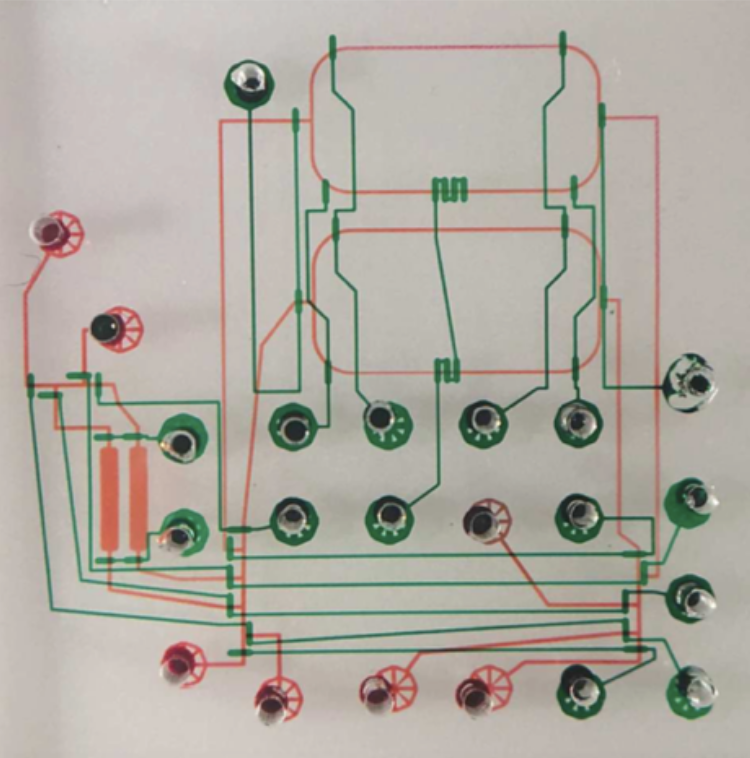
\includegraphics[height = 5cm]{mlsi}
\label{fig:mlsi}
\end{SCfigure}

\section{Overview of the Project}
This project aims to develop a prototype of mLSI simulator. Formally:
\paragraph{Input}
\begin{itemize}
\item A description of the physical structure of an mLSI chip (.txt file);
\item A description of the application protocols (txt.file);
\item A specific time point (a floating point number).
\end{itemize}
\paragraph{Output}
\begin{itemize}
\item The channel status, i.e. whether it is blocked, vacant or filled with fluids, at a specific time point (txt.file).
\end{itemize}

\begin{figure}
\caption{System diagram of the Project}
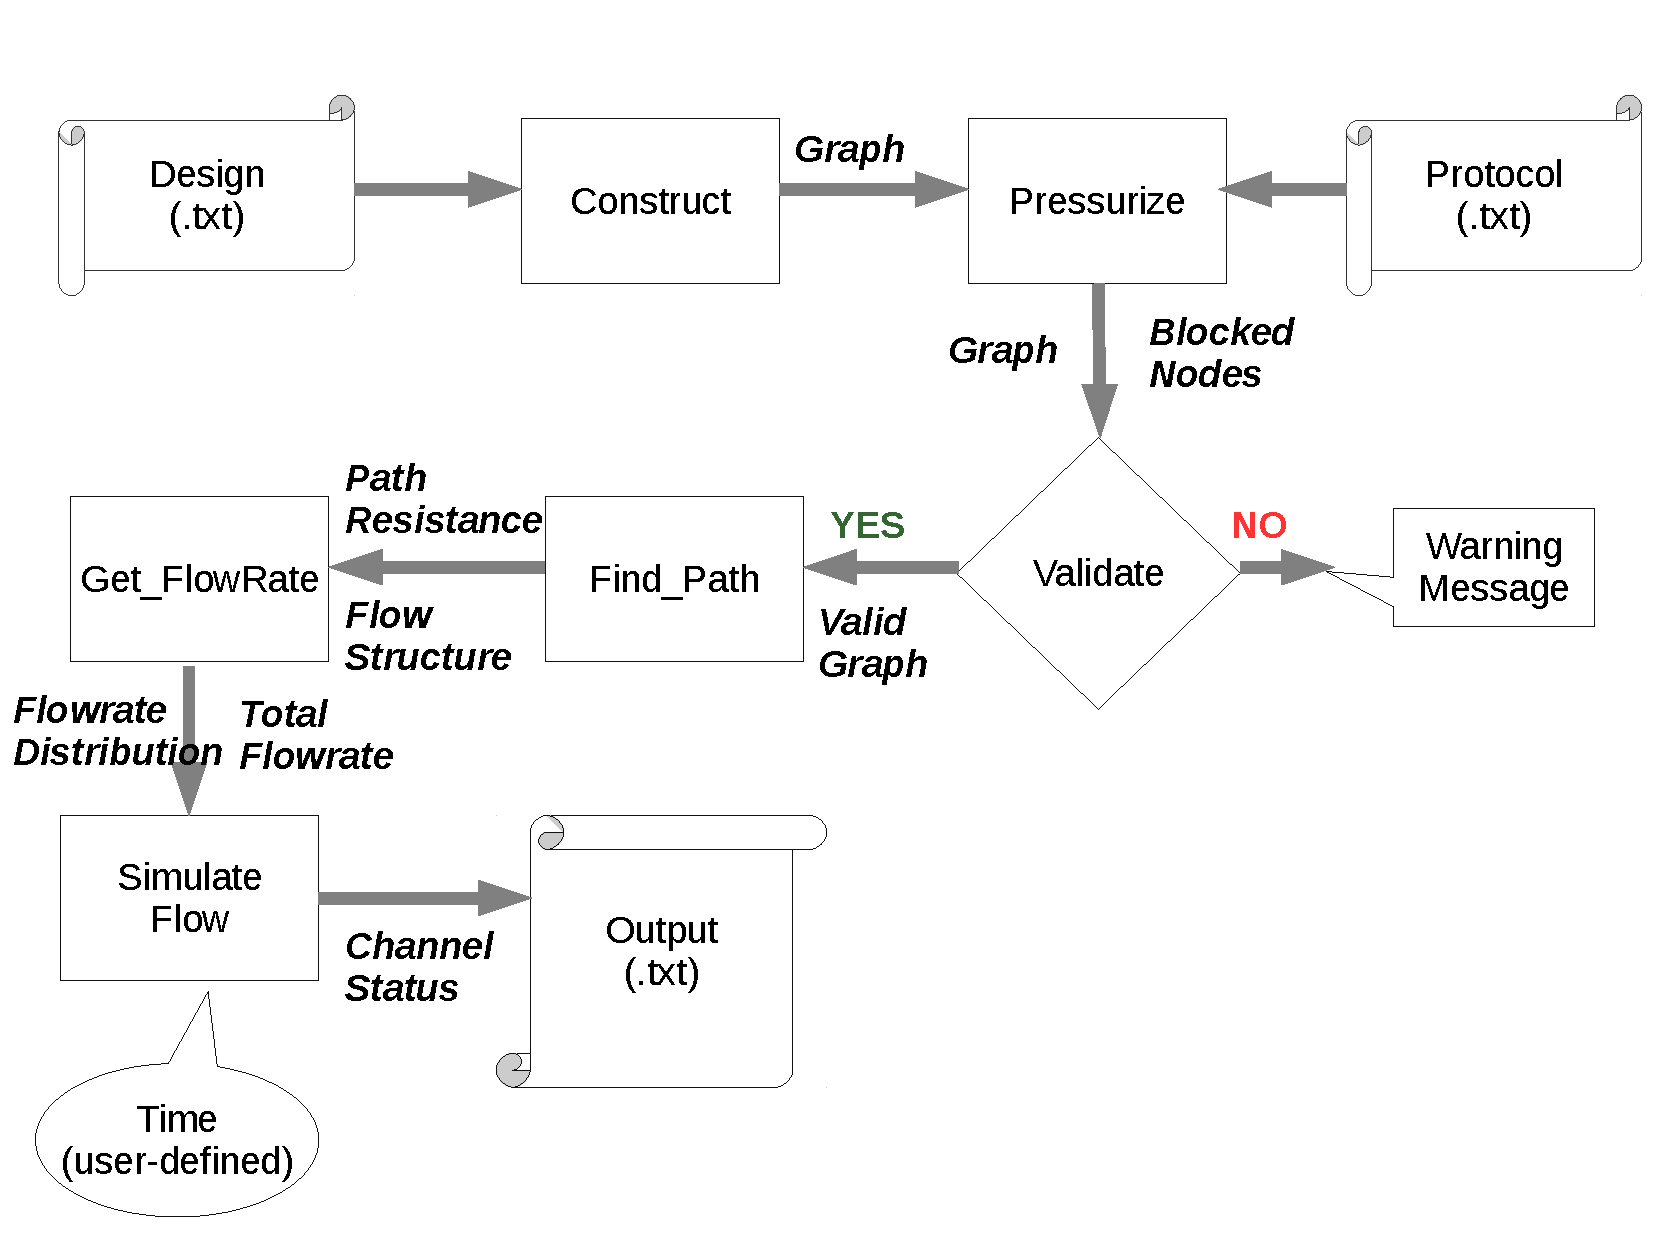
\includegraphics[height = 8cm]{systemdiagram}
\label{fig:system}
\end{figure}

Figure~\ref{fig:system} shows the system diagram of the simulator. 
The simulator first takes a description of the chip \textit{design} as its input, and \textit{constructs} a \textbf{graph} structure consisting of nodes and edges. Each node may represent an inlet, an outlet, a valve, or a channel branching point of the mLSI chip, and each edge represents a channel segment that connects two nodes.
After that, the simulator reads a description of application \textit{protocols},
based on which some of the control channels will be \textit{pressurize}d,
and thus some nodes will be blocked.
The \textbf{graph} and the \textbf{blocked nodes} are then fed to the next process that \textit{validate}s whether there is any feasible flow paths on the chip.
If there is no feasible flow path, the simulator will output a \textit{warning message} and terminate. If there is one or more feasible flow paths, the simulator will generate a \textbf{valid graph} where blocked nodes and channels are removed.
Based on the valid graph, the simulator will \textit{find} the directed flow \textit{paths} and calculate their resistance. The \textbf{flow structure } and the \textbf{path resistance} are then used to \textit{get} the \textbf{flow rate distribution} of each edge as well as the \textbf{total flow rate} of the chip. Finally, the simulator \textit{simulates} the fluid \textit{flow} by outputting a text file describing the \textbf{channel status}.

Each rectangle in the system diagram represents a major function in the program, and the arrows going in to and going out from the rectangles are denoted with the input and the output of these functions, respectively.

\begin{figure}
\caption{Code demonstration of the system diagram}
\includegraphics[width = \textwidth]{main}
\label{fig:code_main}
\end{figure}

Figure~\ref{fig:code_main} demonstrates the implementation of the system diagram as codes.

\section{Insight into the Program}

The program is implemented based on a \textbf{graph} concept,
which models the chip structure as well as the flow paths.

A graph consists of two essential members, namely nodes and edges. A graph is called \textit{valid}, if it consists of a valid sequence of edges that connects an inlet node to its destined nodes.

From the algorithmic aspect, there are three essential functions based on graph parameters: \textit{validate}, \textit{find$\_$path}, and \textit{simulate$\_$flow}.
In the following I will explain these functions in more detail. 

\subsection{Validate}

\begin{figure}
\caption{Code demonstration of the validate function.}
\includegraphics[width = \textwidth]{validate}
\label{fig:code_validate}
\end{figure}

Figure~\ref{fig:code_validate} demonstrates the implementation of the validate function.
The validate function takes two input parameters, namely a graph and a container of blocked nodes.
A new graph object will be initialized based on the unblocked nodes in the graph.
Once a node is blocked, the edge connected to it will also be blocked;
and once an edge is blocked, the other node of this edge will also be blocked, unless this node is at a channel branching point.
What's more, if a node which is neither an inlet nor an outlet node, and it is connected to only one edge, there is no way for this node to form a valid flow path and thus it can also be considered as blocked.
This can be referred to the \textit{propagation of the blocked status}. 
The validate functions applies an iterative process to find all the blocked nodes and edges.
Besides, if a node is connected to exactly two edges,
it indicates that the node is an intermediate node of a longer edge.
In this case, the delete$\_$intermediate$\_$node function will update the graph by merging the edges into a new edge and deleting the intermediate node.

\subsection{Find$\_$Path}
\begin{figure}
\caption{Code demonstration of the find$\_$path function.}
\includegraphics[width = \textwidth]{findpath}
\label{fig:findpath}
\end{figure}

Figure~\ref{fig:findpath} demonstrates the implementation of the find$\_$path function. This function takes a valid graph as input parameter and outputs a tuple that specifies both the flow structure and the flow resistance of the edges.
The solution is implemented in an iterative manner. First, if two edges share the same end nodes, it means that these two edges are in parallel.
In this case, these edges can be considered as a wider edge with relatively smaller resistance.
Thus, the simulator will merge the two edges as a new edge with re-calculated flow resistance.
After merging the edges that are in parallel, there can be sequentially connected edges which did not exist in the input valid graph.
Thus,
the simulator will merge these sequentially connected edges and delete the intermediate node.
This action might again introduce new edges that are in parallel,
and thus the iteratively refinement process will only terminate when no more edges can be merged.
In this process, we will keep updating the resistance of the edges, and record all the edges generate intermediately to keep a track of the flow structure.

\subsection{Simulate$\_$Flow}

\begin{figure}
\caption{Code demonstration of the simulate$\_$flow function.}
\includegraphics[width = \textwidth]{simulateflow}
\label{fig:simulateflow}
\end{figure}

Figure~\ref{fig:simulateflow} demonstrates the implementation of the simulate$\_$flow function.
This function takes the records of the flow rate and the graph as its inputs, together with a user defined time parameter.
Based on the time parameter, the simulator calculates the total volume of fluids that can be injected into the chip in the given time interval.
Based on the flow structure, the transportation paths of the fluids are known.
Thus, the simulation starts from the departure node and the edge connected to it.
If the the volume of the fluids surpasses the capacity of the channel represented by this edge,
we know that the fluids will proceed to the next edges connecting to this edge.
If an edge is connected to more than one channels,
the distribution of the fluids into these edges will follow the distribution of the flow rates.
This process repeats until the remained fluids are not enough to fill a given edge.
In this case,
we record the percentage of the fluids to the capacity of the edge. 

\section{Conclusion and Future Work}

The proposed simulator is able to simulate the fluid flow on mLSI chips at a given time point based on the chip design and the application protocols. Currently the simulation results are text files and cannot be interpreted simultaneously. The next step is to develop a visualization method to demonstrate the results. Besides, from functional aspect, the simulation tool is expected to support dynamically adjustments of the protocols.



\end{document}